% Created 2017-09-27 Wed 20:56
% Intended LaTeX compiler: pdflatex
\documentclass[presentation, bigger]{beamer}
\usepackage[no-math]{fontspec}
\usepackage[BoldFont,SlantFont,AutoFakeBold=true,AutoFakeSlant=true]{xeCJK}
\setCJKmainfont[BoldFont=FandolSong-Bold.otf,ItalicFont=FandolKai-Regular.otf]{FandolSong-Regular.otf}
\setCJKsansfont[BoldFont=FandolHei-Bold.otf]{FandolHei-Regular.otf}
\setCJKmonofont{FandolFang-Regular.otf}
\usefonttheme[stillsansseriflarge,stillsansserifsmall]{serif}
\usepackage{graphicx}
\usepackage{xcolor}
\usepackage{listings}
\defaultfontfeatures{Mapping=tex-text}
\usepackage{geometry}
\usepackage{verbatim}
\usepackage{fixltx2e}
\usepackage{longtable}
\usepackage{float}
\usepackage{wrapfig}
\usepackage{rotating}
\usepackage[normalem]{ulem}
\usepackage{amsmath}
\usepackage{marvosym}
\usepackage{wasysym}
\usepackage{amssymb}
\usepackage{hyperref}
\setlength{\parindent}{0in}
\tolerance=1000
\usetheme{metropolis}
\author{刘恩泽}
\date{2017-09-24}
\title{写一个解释器}
\hypersetup{
 pdfauthor={刘恩泽},
 pdftitle={写一个解释器},
 pdfkeywords={},
 pdfsubject={},
 pdfcreator={Emacs 25.3.1 (Org mode 9.1.1)},
 pdflang={English}}
\begin{document}

\maketitle
\begin{frame}{目录}
\tableofcontents
\end{frame}


\section{什么是解释器}
\label{sec:orgabd5bd5}
\begin{frame}[fragile,label={sec:org3533937}]{解释器}
 \begin{itemize}
\item \texttt{同声传译}
\item 一段能够理解并执行 \texttt{你的程序} 的 \texttt{程序}
\begin{itemize}
\item 理解你的代码所表示的意图
\item 执行你的意图
\end{itemize}
\end{itemize}
\end{frame}

\begin{frame}[fragile,label={sec:orgf3baafe}]{代码的意图}
 \begin{itemize}
\item 赋值/定义

\lstset{frame=single,backgroundcolor=\color[gray]{0.95},identifierstyle=\ttfamily,keywordstyle=\color[rgb]{0,0,1},commentstyle=\color[rgb]{0.133,0.545,0.133},stringstyle=\color[rgb]{0.627,0.126,0.941},basicstyle=\scriptsize,extendedchars=true,breaklines=true,prebreak=\raisebox{0ex}[0ex][0ex]{\ensuremath{\hookleftarrow}},columns=fixed,keepspaces=true,showstringspaces=false,numbers=left,xleftmargin=.25in,xrightmargin=.25in,numberstyle=\tiny,language=Lisp,label= ,caption= ,captionpos=b}
\begin{lstlisting}
(setf a 1)
(defun plus (a b) (+ a b))
\end{lstlisting}

\item 取值

\texttt{a}

\item 执行

\texttt{(plus 1 2)}
\end{itemize}
\end{frame}

\begin{frame}[fragile,label={sec:org17ed4b8}]{\texttt{LISP}}
 \begin{block}{\texttt{语法(S Expression)}}
\begin{itemize}
\item 原子 \texttt{a}, \texttt{1}, \texttt{"hello world"}
\item 表 \texttt{()}, \texttt{nil}, \texttt{(a 1 2)}, \texttt{(a . b)} , \texttt{(a . nil)}, \texttt{(a (b))}
\end{itemize}
\end{block}
\begin{block}{\texttt{语义}}
\begin{description}
\item[{原子表达式}] 即 \texttt{a}, \texttt{1} 等原子,可直接求值或上下文中查找对应的值
\item[{复合表达式}] 函数
\item[{特殊形式}] 求值方式与函数不一致
\end{description}
\end{block}
\end{frame}

\section{如何下手}
\label{sec:org58d33f0}
\begin{frame}[fragile,allowframebreaks,label=]{步骤}
 \alert{Dragon book}, 中文名 \texttt{编译原理}
\begin{center}
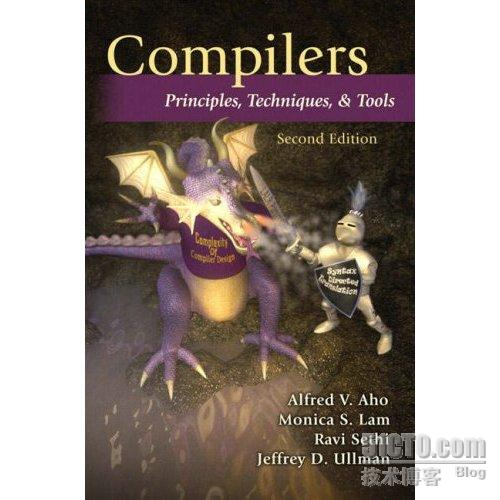
\includegraphics[width=0.5\textwidth]{./img/dragon.jpg}
\end{center}

\framebreak
\alert{Tiger book}, 中文名 \texttt{现代编译原理-C 语言描述}
\begin{center}

\includegraphics[width=0.3\textwidth]{./img/tiger.jpg}
\end{center}

\framebreak

\alert{Whale book}, 中文名 \texttt{高级编译器设计与实现}
\begin{center}

\includegraphics[width=0.3\textwidth]{./img/whale.jpg}
\end{center}
\end{frame}

\begin{frame}[label={sec:orga8944f3}]{结束}
\begin{itemize}
\item <+-> 好,分享结束,大家可以回去看书了.
\item <2-> 预计一年后,应该可以成功写出来了。
\item <3> 开个玩笑,我们继续. 看一个 \alert{半小时就能写出来的版本} 。
\end{itemize}
\end{frame}

\section{半小时版本}
\label{sec:org701a80c}
\begin{frame}[label={sec:org2d32788}]{核心逻辑}
\begin{itemize}
\item parse -> (eval\footnote{处理表达式} -> apply\footnote{处理值}) loop\ldots{}
\end{itemize}
\begin{center}
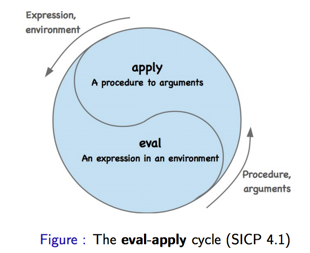
\includegraphics[width=0.3\textwidth]{./img/eval-apply.png}
\end{center}
\end{frame}
\begin{frame}[fragile,label={sec:orgaa054ab}]{解析(1 min)}
 这里我们就偷个懒,利用 \texttt{lisp} 的 \texttt{read-from-string} / \texttt{read} 方法

\lstset{frame=single,backgroundcolor=\color[gray]{0.95},identifierstyle=\ttfamily,keywordstyle=\color[rgb]{0,0,1},commentstyle=\color[rgb]{0.133,0.545,0.133},stringstyle=\color[rgb]{0.627,0.126,0.941},basicstyle=\scriptsize,extendedchars=true,breaklines=true,prebreak=\raisebox{0ex}[0ex][0ex]{\ensuremath{\hookleftarrow}},columns=fixed,keepspaces=true,showstringspaces=false,numbers=left,xleftmargin=.25in,xrightmargin=.25in,numberstyle=\tiny,language=Lisp,label= ,caption= ,captionpos=b}
\begin{lstlisting}
(read-from-string "(1 2 3)")
;;; => (1 2 3)
(read-from-string "1")
;;; => 1
(read-from-string "nil")
 ;;; => NIL
(read-from-string "(defun plus (a b ) (+ a b))")
;;; => (DEFUN PLUS (A B) (+ A B))
(read-from-string "(defun plus (a b)")
;;; Exception
\end{lstlisting}
\end{frame}

\begin{frame}[label={sec:org8cf6684}]{表达式类型}
\begin{itemize}
\item 原子
\begin{itemize}
\item 常量 \alert{1}, \alert{"abc"}
\item 变量 \alert{a}, \alert{test}
\end{itemize}
\item 列表
\begin{itemize}
\item quote \alert{(quote (a b c))}
\item if \alert{(if t 1 2)}
\item lambda \alert{(lambda (a) (+ 1 a))}
\item define \alert{(define a 1)}
\item assign \alert{(set! a 2)}
\item begin \alert{(begin (define b 1) (set! b 2))}
\item apply procedure \alert{(plus 1 2)}
\end{itemize}
\end{itemize}
\end{frame}

\begin{frame}[fragile,label={sec:orga68c5b0}]{原子表达式}
 \begin{block}{符号}
\begin{quote}
\texttt{当遇到了一个符号的时候,从当前的上下文中去查找其对应的值,做替换}
\end{quote}

\lstset{frame=single,backgroundcolor=\color[gray]{0.95},identifierstyle=\ttfamily,keywordstyle=\color[rgb]{0,0,1},commentstyle=\color[rgb]{0.133,0.545,0.133},stringstyle=\color[rgb]{0.627,0.126,0.941},basicstyle=\scriptsize,extendedchars=true,breaklines=true,prebreak=\raisebox{0ex}[0ex][0ex]{\ensuremath{\hookleftarrow}},columns=fixed,keepspaces=true,showstringspaces=false,numbers=left,xleftmargin=.25in,xrightmargin=.25in,numberstyle=\tiny,language=Lisp,label= ,caption= ,captionpos=b}
\begin{lstlisting}
a ;;; nil or unbound exception
(set! a 1) ;;; => 1
a ;;; => 1
\end{lstlisting}
\end{block}

\begin{block}{常量}
\begin{quote}
\texttt{常量表达式的值即为本身}
\end{quote}

\lstset{frame=single,backgroundcolor=\color[gray]{0.95},identifierstyle=\ttfamily,keywordstyle=\color[rgb]{0,0,1},commentstyle=\color[rgb]{0.133,0.545,0.133},stringstyle=\color[rgb]{0.627,0.126,0.941},basicstyle=\scriptsize,extendedchars=true,breaklines=true,prebreak=\raisebox{0ex}[0ex][0ex]{\ensuremath{\hookleftarrow}},columns=fixed,keepspaces=true,showstringspaces=false,numbers=left,xleftmargin=.25in,xrightmargin=.25in,numberstyle=\tiny,language=Lisp,label= ,caption= ,captionpos=b}
\begin{lstlisting}
1 ;;; => 1
"abc" ;;; "abc"
\end{lstlisting}
\end{block}
\end{frame}

\begin{frame}[fragile,label={sec:orgb2a84e3}]{特殊形式 \alert{if}}
 \lstset{frame=single,backgroundcolor=\color[gray]{0.95},identifierstyle=\ttfamily,keywordstyle=\color[rgb]{0,0,1},commentstyle=\color[rgb]{0.133,0.545,0.133},stringstyle=\color[rgb]{0.627,0.126,0.941},basicstyle=\scriptsize,extendedchars=true,breaklines=true,prebreak=\raisebox{0ex}[0ex][0ex]{\ensuremath{\hookleftarrow}},columns=fixed,keepspaces=true,showstringspaces=false,numbers=left,xleftmargin=.25in,xrightmargin=.25in,numberstyle=\tiny,language=Lisp,label= ,caption= ,captionpos=b}
\begin{lstlisting}
(if predicate consuquence alternative)
\end{lstlisting}

\begin{quote}
先求值 \texttt{predicate} , 如果符合,则求值 \texttt{consquence}, 反之,则求值 \texttt{alternative}
\end{quote}

特殊在于, \texttt{控制表内的求值顺序} 。

并不会将表内表达式均求值,而是根据第一个元素的值,来决定后续如何进行求值。
\end{frame}

\begin{frame}[fragile,label={sec:org276f1f0}]{特殊形式 \alert{define} 以及 \alert{set!}}
 \lstset{frame=single,backgroundcolor=\color[gray]{0.95},identifierstyle=\ttfamily,keywordstyle=\color[rgb]{0,0,1},commentstyle=\color[rgb]{0.133,0.545,0.133},stringstyle=\color[rgb]{0.627,0.126,0.941},basicstyle=\scriptsize,extendedchars=true,breaklines=true,prebreak=\raisebox{0ex}[0ex][0ex]{\ensuremath{\hookleftarrow}},columns=fixed,keepspaces=true,showstringspaces=false,numbers=left,xleftmargin=.25in,xrightmargin=.25in,numberstyle=\tiny,language=Lisp,label= ,caption= ,captionpos=b}
\begin{lstlisting}
(define variable value)
(set! variable value)
\end{lstlisting}

\begin{quote}
只求值 \texttt{value}, 并将求值后的结果赋值给 \texttt{variable}\footnote{赋值表示在上下文中添加 (install) 这个符号以及这个符号对应的值.}
\end{quote}

特殊在于, \texttt{控制表内的求值顺序} 以及 \texttt{修改上下文}

不对 \texttt{variable} 求值,仅求值 \texttt{value}, 而后修改上下文。
\end{frame}

\begin{frame}[fragile,label={sec:org08d36e8}]{特殊形式 \alert{quote}}
 \lstset{frame=single,backgroundcolor=\color[gray]{0.95},identifierstyle=\ttfamily,keywordstyle=\color[rgb]{0,0,1},commentstyle=\color[rgb]{0.133,0.545,0.133},stringstyle=\color[rgb]{0.627,0.126,0.941},basicstyle=\scriptsize,extendedchars=true,breaklines=true,prebreak=\raisebox{0ex}[0ex][0ex]{\ensuremath{\hookleftarrow}},columns=fixed,keepspaces=true,showstringspaces=false,numbers=left,xleftmargin=.25in,xrightmargin=.25in,numberstyle=\tiny,language=Lisp,label= ,caption= ,captionpos=b}
\begin{lstlisting}
(quote (a b c))
\end{lstlisting}

\begin{quote}
返回其引用的表达式
\end{quote}

syntactic sugar: \texttt{'(a b c)}

特殊在于, \texttt{控制表内的求值顺序} 。

不对表达式内求值,仅返回其引用的表达式。
\end{frame}

\begin{frame}[fragile,label={sec:org99749ca}]{特殊形式 \alert{lambda}}
 \lstset{frame=single,backgroundcolor=\color[gray]{0.95},identifierstyle=\ttfamily,keywordstyle=\color[rgb]{0,0,1},commentstyle=\color[rgb]{0.133,0.545,0.133},stringstyle=\color[rgb]{0.627,0.126,0.941},basicstyle=\scriptsize,extendedchars=true,breaklines=true,prebreak=\raisebox{0ex}[0ex][0ex]{\ensuremath{\hookleftarrow}},columns=fixed,keepspaces=true,showstringspaces=false,numbers=left,xleftmargin=.25in,xrightmargin=.25in,numberstyle=\tiny,language=Lisp,label= ,caption= ,captionpos=b}
\begin{lstlisting}
(lambda (a) (+ 1 a))
\end{lstlisting}

\begin{quote}
生成一个 \texttt{procedure}, 包含 \alert{形式参数} 列表,以及 \alert{待执行的表达式} 列表。
\end{quote}

特殊同样在于, \texttt{控制表内的求值顺序} 。

只将待执行的表达式记录下来,留待需要时使用。
\end{frame}

\begin{frame}[fragile,label={sec:org8af9dc8}]{特殊形式 \alert{begin}}
 \lstset{frame=single,backgroundcolor=\color[gray]{0.95},identifierstyle=\ttfamily,keywordstyle=\color[rgb]{0,0,1},commentstyle=\color[rgb]{0.133,0.545,0.133},stringstyle=\color[rgb]{0.627,0.126,0.941},basicstyle=\scriptsize,extendedchars=true,breaklines=true,prebreak=\raisebox{0ex}[0ex][0ex]{\ensuremath{\hookleftarrow}},columns=fixed,keepspaces=true,showstringspaces=false,numbers=left,xleftmargin=.25in,xrightmargin=.25in,numberstyle=\tiny,language=Lisp,label= ,caption= ,captionpos=b}
\begin{lstlisting}
(begin
 (define a 3)
 (set! a 1)
 (+ a 2))
\end{lstlisting}

\begin{quote}
依次执行表达式序列
\end{quote}

特殊在于, \texttt{控制表内的求值顺序}
\end{frame}

\begin{frame}[fragile,allowframebreaks,label=]{函数调用}
 \lstset{frame=single,backgroundcolor=\color[gray]{0.95},identifierstyle=\ttfamily,keywordstyle=\color[rgb]{0,0,1},commentstyle=\color[rgb]{0.133,0.545,0.133},stringstyle=\color[rgb]{0.627,0.126,0.941},basicstyle=\scriptsize,extendedchars=true,breaklines=true,prebreak=\raisebox{0ex}[0ex][0ex]{\ensuremath{\hookleftarrow}},columns=fixed,keepspaces=true,showstringspaces=false,numbers=left,xleftmargin=.25in,xrightmargin=.25in,numberstyle=\tiny,language=Lisp,label= ,caption= ,captionpos=b}
\begin{lstlisting}
(define plus (lambda (a) (+ 1 a)))
(plus 2) ;;; 3
\end{lstlisting}

\begin{quote}
\begin{enumerate}
\item 求值操作符
\item 求值操作数
\item 应用该操作
\begin{itemize}
\item 系统方法,则直接调用下层的 apply
\item 自定义的方法
\begin{enumerate}
\item 把形参对应的值添加到上下文中, 生成新的上下文
\item 在新的上下文中,求值表达式列表
\end{enumerate}
\end{itemize}
\end{enumerate}
\end{quote}

\framebreak

函数定义

\lstset{frame=single,backgroundcolor=\color[gray]{0.95},identifierstyle=\ttfamily,keywordstyle=\color[rgb]{0,0,1},commentstyle=\color[rgb]{0.133,0.545,0.133},stringstyle=\color[rgb]{0.627,0.126,0.941},basicstyle=\scriptsize,extendedchars=true,breaklines=true,prebreak=\raisebox{0ex}[0ex][0ex]{\ensuremath{\hookleftarrow}},columns=fixed,keepspaces=true,showstringspaces=false,numbers=left,xleftmargin=.25in,xrightmargin=.25in,numberstyle=\tiny,language=Lisp,label= ,caption= ,captionpos=b}
\begin{lstlisting}
;;; env => ((+) (<primitive +>))
(define plus1 (lambda (a) (+ 1 a)))
;;; env =>
;;;       ( (+ plus1)
;;;         (<primitive +> <procedure object>) )

(plus1 2)
\end{lstlisting}

\framebreak

执行过程

\lstset{frame=single,backgroundcolor=\color[gray]{0.95},identifierstyle=\ttfamily,keywordstyle=\color[rgb]{0,0,1},commentstyle=\color[rgb]{0.133,0.545,0.133},stringstyle=\color[rgb]{0.627,0.126,0.941},basicstyle=\scriptsize,extendedchars=true,breaklines=true,prebreak=\raisebox{0ex}[0ex][0ex]{\ensuremath{\hookleftarrow}},columns=fixed,keepspaces=true,showstringspaces=false,numbers=left,xleftmargin=.25in,xrightmargin=.25in,numberstyle=\tiny,language=Lisp,label= ,caption= ,captionpos=b}
\begin{lstlisting}
(eval 'plus1 env) ;;; <procedure object>
(eval 2) ;;; 2
(extend (a) (2) env)
;;; env' => ( (+ plus1 a)
;;;           (<primitive +> <procedure object> 2))

(eval '(+ 1 a) env')
(eval a env') ;;; 2
(apply-primitive '+ (1 2)) ;;; 3
\end{lstlisting}
\end{frame}

\begin{frame}[label={sec:orgc5c3e7c}]{求值环境/上下文}
\begin{center}
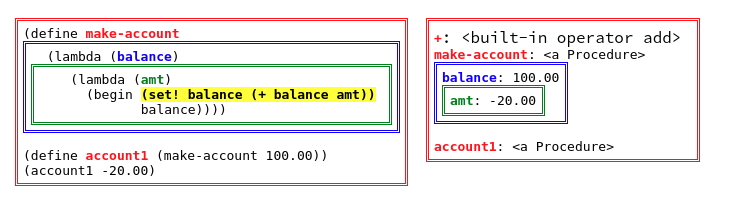
\includegraphics[width=.9\linewidth]{./img/context.png}
\end{center}
\end{frame}

\section{实现一个解释器}
\label{sec:org243fb4b}
\begin{frame}[label={sec:orge1c8c53}]{声明}
源代码来自 SICP 第 4 章,链接见附录。
\end{frame}

\begin{frame}[fragile,label={sec:org05cf57d}]{\texttt{eval} (dispatch)}
 \lstset{frame=single,backgroundcolor=\color[gray]{0.95},identifierstyle=\ttfamily,keywordstyle=\color[rgb]{0,0,1},commentstyle=\color[rgb]{0.133,0.545,0.133},stringstyle=\color[rgb]{0.627,0.126,0.941},basicstyle=\scriptsize,extendedchars=true,breaklines=true,prebreak=\raisebox{0ex}[0ex][0ex]{\ensuremath{\hookleftarrow}},columns=fixed,keepspaces=true,showstringspaces=false,numbers=left,xleftmargin=.25in,xrightmargin=.25in,numberstyle=\tiny,language=Lisp,label= ,caption= ,captionpos=b}
\begin{lstlisting}
(define (eval exp env)
  (cond ((self-evaluating? exp) exp)
        ((variable? exp) (lookup-variable-value exp env))
        ((quoted? exp) (text-of-quotation exp))
        ((assignment? exp) (eval-assignment exp env))
        ((definition? exp) (eval-definition exp env))
        ((if? exp) (eval-if exp env))
        ((lambda? exp)
         (make-procedure (lambda-parameters exp)
                         (lambda-body exp)
                         env))
        ((begin? exp)
         (eval-sequence (begin-actions exp) env))
        ((application? exp)
         (apply (eval (operator exp) env)
                (list-of-values (operands exp) env)))
        (else
         (error "Unknown expression type -- EVAL" exp))))
\end{lstlisting}
\end{frame}
\begin{frame}[fragile,label={sec:org5a135bf}]{\texttt{apply}}
 \lstset{frame=single,backgroundcolor=\color[gray]{0.95},identifierstyle=\ttfamily,keywordstyle=\color[rgb]{0,0,1},commentstyle=\color[rgb]{0.133,0.545,0.133},stringstyle=\color[rgb]{0.627,0.126,0.941},basicstyle=\scriptsize,extendedchars=true,breaklines=true,prebreak=\raisebox{0ex}[0ex][0ex]{\ensuremath{\hookleftarrow}},columns=fixed,keepspaces=true,showstringspaces=false,numbers=left,xleftmargin=.25in,xrightmargin=.25in,numberstyle=\tiny,language=Lisp,label= ,caption= ,captionpos=b}
\begin{lstlisting}
(define (apply procedure arguments)
  (cond ((primitive-procedure? procedure)
         (apply-primitive-procedure procedure arguments))
        ((compound-procedure? procedure)
         (eval-sequence
           (procedure-body procedure)
           (extend-environment
             (procedure-parameters procedure)
             arguments
             (procedure-environment procedure))))
        (else
         (error
          "Unknown procedure type -- APPLY" procedure))))
\end{lstlisting}
\end{frame}
\begin{frame}[fragile,allowframebreaks,label=]{\texttt{env} 求值上下文}
 \lstset{frame=single,backgroundcolor=\color[gray]{0.95},identifierstyle=\ttfamily,keywordstyle=\color[rgb]{0,0,1},commentstyle=\color[rgb]{0.133,0.545,0.133},stringstyle=\color[rgb]{0.627,0.126,0.941},basicstyle=\scriptsize,extendedchars=true,breaklines=true,prebreak=\raisebox{0ex}[0ex][0ex]{\ensuremath{\hookleftarrow}},columns=fixed,keepspaces=true,showstringspaces=false,numbers=left,xleftmargin=.25in,xrightmargin=.25in,numberstyle=\tiny,language=Lisp,label= ,caption= ,captionpos=b}
\begin{lstlisting}
(define (enclosing-environment env) (cdr env))
(define (first-frame env) (car env))
(define the-empty-environment '())

(define (make-frame variables values)
  (cons variables values))
(define (frame-variables frame) (car frame))
(define (frame-values frame) (cdr frame))
(define (add-binding-to-frame! var val frame)
  (set-car! frame (cons var (car frame)))
  (set-cdr! frame (cons val (cdr frame))))
\end{lstlisting}

\framebreak
\lstset{frame=single,backgroundcolor=\color[gray]{0.95},identifierstyle=\ttfamily,keywordstyle=\color[rgb]{0,0,1},commentstyle=\color[rgb]{0.133,0.545,0.133},stringstyle=\color[rgb]{0.627,0.126,0.941},basicstyle=\scriptsize,extendedchars=true,breaklines=true,prebreak=\raisebox{0ex}[0ex][0ex]{\ensuremath{\hookleftarrow}},columns=fixed,keepspaces=true,showstringspaces=false,numbers=left,xleftmargin=.25in,xrightmargin=.25in,numberstyle=\tiny,language=Lisp,label= ,caption= ,captionpos=b}
\begin{lstlisting}
(define (extend-environment vars vals base-env)
  (if (= (length vars) (length vals))
      (cons (make-frame vars vals) base-env)
      (if (< (length vars) (length vals))
          (error "Too many arguments supplied" vars vals)
          (error "Too few arguments supplied" vars vals))))

\end{lstlisting}
\end{frame}

\begin{frame}[fragile,allowframebreaks,label=]{\texttt{eval-atom}}
 \lstset{frame=single,backgroundcolor=\color[gray]{0.95},identifierstyle=\ttfamily,keywordstyle=\color[rgb]{0,0,1},commentstyle=\color[rgb]{0.133,0.545,0.133},stringstyle=\color[rgb]{0.627,0.126,0.941},basicstyle=\scriptsize,extendedchars=true,breaklines=true,prebreak=\raisebox{0ex}[0ex][0ex]{\ensuremath{\hookleftarrow}},columns=fixed,keepspaces=true,showstringspaces=false,numbers=left,xleftmargin=.25in,xrightmargin=.25in,numberstyle=\tiny,language=Lisp,label= ,caption= ,captionpos=b}
\begin{lstlisting}
(define (self-evaluating? exp)
  (cond ((number? exp) true)
        ((string? exp) true)
        (else false)))

(define (variable? exp) (symbol? exp))

\end{lstlisting}

\framebreak
\lstset{frame=single,backgroundcolor=\color[gray]{0.95},identifierstyle=\ttfamily,keywordstyle=\color[rgb]{0,0,1},commentstyle=\color[rgb]{0.133,0.545,0.133},stringstyle=\color[rgb]{0.627,0.126,0.941},basicstyle=\scriptsize,extendedchars=true,breaklines=true,prebreak=\raisebox{0ex}[0ex][0ex]{\ensuremath{\hookleftarrow}},columns=fixed,keepspaces=true,showstringspaces=false,numbers=left,xleftmargin=.25in,xrightmargin=.25in,numberstyle=\tiny,language=Lisp,label= ,caption= ,captionpos=b}
\begin{lstlisting}
(define (lookup-variable-value var env)
  (define (env-loop env)
    (define (scan vars vals)
      (cond ((null? vars)
             (env-loop (enclosing-environment env)))
            ((eq? var (car vars))
             (car vals))
            (else (scan (cdr vars) (cdr vals)))))
    (if (eq? env the-empty-environment)
        (error "Unbound variable" var)
        (let ((frame (first-frame env)))
          (scan (frame-variables frame)
                (frame-values frame)))))
  (env-loop env))
\end{lstlisting}
\end{frame}


\begin{frame}[fragile,allowframebreaks,label=]{\texttt{eval-define} \& \texttt{eval-assign}}
 \lstset{frame=single,backgroundcolor=\color[gray]{0.95},identifierstyle=\ttfamily,keywordstyle=\color[rgb]{0,0,1},commentstyle=\color[rgb]{0.133,0.545,0.133},stringstyle=\color[rgb]{0.627,0.126,0.941},basicstyle=\scriptsize,extendedchars=true,breaklines=true,prebreak=\raisebox{0ex}[0ex][0ex]{\ensuremath{\hookleftarrow}},columns=fixed,keepspaces=true,showstringspaces=false,numbers=left,xleftmargin=.25in,xrightmargin=.25in,numberstyle=\tiny,language=Lisp,label= ,caption= ,captionpos=b}
\begin{lstlisting}
(define (eval-assignment exp env)
  (set-variable-value!
     (assignment-variable exp)
     (eval (assignment-value exp) env)
     env)
  'ok)

(define (eval-definition exp env)
    (define-variable!
        (definition-variable exp)
        (eval (definition-value exp) env)
      env)
  'ok)
\end{lstlisting}

\framebreak
\lstset{frame=single,backgroundcolor=\color[gray]{0.95},identifierstyle=\ttfamily,keywordstyle=\color[rgb]{0,0,1},commentstyle=\color[rgb]{0.133,0.545,0.133},stringstyle=\color[rgb]{0.627,0.126,0.941},basicstyle=\scriptsize,extendedchars=true,breaklines=true,prebreak=\raisebox{0ex}[0ex][0ex]{\ensuremath{\hookleftarrow}},columns=fixed,keepspaces=true,showstringspaces=false,numbers=left,xleftmargin=.25in,xrightmargin=.25in,numberstyle=\tiny,language=Lisp,label= ,caption= ,captionpos=b}
\begin{lstlisting}
(define (define-variable! var val env)
  (let ((frame (first-frame env)))
    (define (scan vars vals)
      (cond ((null? vars)
             (add-binding-to-frame! var val frame))
            ((eq? var (car vars))
             (set-car! vals val))
            (else (scan (cdr vars) (cdr vals)))))
    (scan (frame-variables frame)
          (frame-values frame))))
\end{lstlisting}
\end{frame}

\begin{frame}[fragile,label={sec:org35c33d7}]{\texttt{eval-if}}
 \lstset{frame=single,backgroundcolor=\color[gray]{0.95},identifierstyle=\ttfamily,keywordstyle=\color[rgb]{0,0,1},commentstyle=\color[rgb]{0.133,0.545,0.133},stringstyle=\color[rgb]{0.627,0.126,0.941},basicstyle=\scriptsize,extendedchars=true,breaklines=true,prebreak=\raisebox{0ex}[0ex][0ex]{\ensuremath{\hookleftarrow}},columns=fixed,keepspaces=true,showstringspaces=false,numbers=left,xleftmargin=.25in,xrightmargin=.25in,numberstyle=\tiny,language=Lisp,label= ,caption= ,captionpos=b}
\begin{lstlisting}
(define (eval-if exp env)
  (if (true? (eval (if-predicate exp) env))
      (eval (if-consequent exp) env)
      (eval (if-alternative exp) env)))

\end{lstlisting}
\end{frame}
\begin{frame}[fragile,label={sec:orgad3fc64}]{\texttt{eval-quote}}
 \lstset{frame=single,backgroundcolor=\color[gray]{0.95},identifierstyle=\ttfamily,keywordstyle=\color[rgb]{0,0,1},commentstyle=\color[rgb]{0.133,0.545,0.133},stringstyle=\color[rgb]{0.627,0.126,0.941},basicstyle=\scriptsize,extendedchars=true,breaklines=true,prebreak=\raisebox{0ex}[0ex][0ex]{\ensuremath{\hookleftarrow}},columns=fixed,keepspaces=true,showstringspaces=false,numbers=left,xleftmargin=.25in,xrightmargin=.25in,numberstyle=\tiny,language=Lisp,label= ,caption= ,captionpos=b}
\begin{lstlisting}
(define (quoted? exp)
  (tagged-list? exp 'quote))

(define (text-of-quotation exp) (cadr exp))

\end{lstlisting}
\end{frame}
\begin{frame}[fragile,label={sec:orga8788b0}]{\texttt{eval-lambda}}
 \lstset{frame=single,backgroundcolor=\color[gray]{0.95},identifierstyle=\ttfamily,keywordstyle=\color[rgb]{0,0,1},commentstyle=\color[rgb]{0.133,0.545,0.133},stringstyle=\color[rgb]{0.627,0.126,0.941},basicstyle=\scriptsize,extendedchars=true,breaklines=true,prebreak=\raisebox{0ex}[0ex][0ex]{\ensuremath{\hookleftarrow}},columns=fixed,keepspaces=true,showstringspaces=false,numbers=left,xleftmargin=.25in,xrightmargin=.25in,numberstyle=\tiny,language=Lisp,label= ,caption= ,captionpos=b}
\begin{lstlisting}
(define (make-procedure parameters body env)
  (list 'procedure parameters body env))
(define (compound-procedure? p)
  (tagged-list? p 'procedure))
(define (procedure-parameters p) (cadr p))
(define (procedure-body p) (caddr p))
(define (procedure-environment p) (cadddr p))
\end{lstlisting}
\end{frame}
\begin{frame}[fragile,label={sec:org3c9ad0a}]{\texttt{eval-begin}}
 \lstset{frame=single,backgroundcolor=\color[gray]{0.95},identifierstyle=\ttfamily,keywordstyle=\color[rgb]{0,0,1},commentstyle=\color[rgb]{0.133,0.545,0.133},stringstyle=\color[rgb]{0.627,0.126,0.941},basicstyle=\scriptsize,extendedchars=true,breaklines=true,prebreak=\raisebox{0ex}[0ex][0ex]{\ensuremath{\hookleftarrow}},columns=fixed,keepspaces=true,showstringspaces=false,numbers=left,xleftmargin=.25in,xrightmargin=.25in,numberstyle=\tiny,language=Lisp,label= ,caption= ,captionpos=b}
\begin{lstlisting}
(define (eval-sequence exps env)
  (cond ((last-exp? exps) (eval (first-exp exps) env))
        (else (eval (first-exp exps) env)
              (eval-sequence (rest-exps exps) env))))
\end{lstlisting}
\end{frame}

\section{最后}
\label{sec:orgbe5e397}
\begin{frame}[fragile,label={sec:orga1eecfe}]{几个题外话}
 \begin{itemize}
\item 如果没有 assign, 会不会简单很多
\item 如果使用 lazy 的求值, 而不是应用时求值,是否很多特殊形式就没有必要了
\item 如果增加一个 \texttt{case} 的关键字
\item 如果做语法分析
\item 如果要编译成 c
\end{itemize}
\end{frame}

\begin{frame}[label={sec:orgcb5f36b}]{参考文档}
\begin{itemize}
\item \href{http://norvig.com/lispy.html}{(How to Write a (Lisp) Interpreter (in Python))}
\item \href{http://norvig.com/lispy2.html}{(An ((Even Better) Lisp) Interpreter (in Python))}
\item \href{https://mitpress.mit.edu/sicp/full-text/book/book-Z-H-26.html\#\%\_sec\_4.1}{SICP Charpter 4: The Metacircular Evaluator}
\end{itemize}
\end{frame}
\end{document}